% !TEX encoding = UTF-8 Unicode
% !TEX spellcheck = en-US


% This is the root file of your thesis: thesis.tex
% A line starting with % is a comment. In some cases, I have included a command preceded by a %. You may activate the command by removing the %.

%%===================================
\documentclass[12pt]{report}
\usepackage{ramsstyle}
\usepackage{diagbox}
\usepackage{array}
%%===================================
%Write the various parts of your thesis as separate files and include them into the main file by the command \include{name of included file}. When you compile the LaTeX file, you may choose which subfiles to include by the command

%\includeonly{chapter01,chapter02}

%%===================================
\begin{document}
% !TEX encoding = UTF-8 Unicode
%!TEX root = thesis.tex
% !TEX spellcheck = en-US

%This is the Titlepage
%%=========================================
\thispagestyle{empty}
\mbox{}\\[6pc]
\begin{center}
\Huge{Porting the HPC-Lab Snow Simulator to OpenCL}\\[2pc]

\Large{Imre Kerr}\\[1pc]
\large{December 2014}\\[2pc]

SPECIALIZATION PROJECT\\
Department of Computer and Information Science\\
Norwegian University of Science and Technology
\end{center}
\vfill

\noindent Supervisor: Dr. Anne C. Elster

 % This is the titlepage
\setcounter{page}{0}
\pagenumbering{roman}
% !TEX encoding = UTF-8 Unicode
%!TEX root = thesis.tex
% !TEX spellcheck = en-US
%%=========================================
\addcontentsline{toc}{section}{Problem Description}
\section*{Problem Description}
OpenCL is a recently defined and widespread open standard that will make the massive parallelism power now available in GPUs, but also newer CPUs (like the Cell B.E.) , more easily accessible to programmers.

This project involves porting an existing OpenCL snow simulation application to Open CL and comparing the implementation and benchmarks to those implemented in CUDA.\\[2cm]

\begin{center}
Trondheim, 2015-01-04\\[1pc]
Supervisor: Dr. Anne C. Elster
\end{center}
% !TEX encoding = UTF-8 Unicode
%!TEX root = thesis.tex
% !TEX spellcheck = en-US
%%=========================================
\addcontentsline{toc}{section}{Acknowledgment}
\section*{Acknowledgment}
I would like to thank Dr. Anne C. Elster for heading the HPC-Lab and giving me the opportunity to work there. The lab provides a unique opportunity for students to work together and learn from each other, all in a great work environment.

I would also like to thank Jørgen Kvalsvik for providing valuable expertise on build systems, in particular CMake.
\begin{flushright}
I.K.\\[1pc]
\end{flushright}
% !TEX encoding = UTF-8 Unicode
%!TEX root = thesis.tex
% !TEX spellcheck = en-US
%%=========================================
\addcontentsline{toc}{section}{Abstract}
\section*{Abstract}
The HPC-Lab Snow Simulator is a computationally demanding physics simulation program which runs on graphics hardware (GPGPU computing). The subject of this project is the porting of this program from the vendor locked-in CUDA API to an open one, OpenCL.

I also evaluate the performance of the resulting program using available profiling tools, and suggest changes which might be done to improve performance based on my findings.
\tableofcontents
\setcounter{page}{0}
\pagenumbering{arabic}
% !TEX encoding = UTF-8 Unicode
%!TEX root = thesis.tex
% !TEX spellcheck = en-US
%%=========================================
\chapter{Introduction}
The first chapter of a well-structured thesis is always an introduction, setting the scene with background, problem description, objectives, limitations, and then looking ahead to summarize what is in the rest of the report. This is the part that readers look at first---\emph{so make sure it hooks them!}

%%=========================================
\section{Background}
In this section, you should present the problem that you are going to investigate or analyze; why this problem is of interest; what has, so far, been done to solve the problem, and which parts of the problem that remain.

{\color{red}Below, I have set up some headings (subsection titles) without a number. These are included to help you remember to cover the related issues. The headings should be removed in your final print.}
%%=========================================
\subsection*{Problem Formulation}
You should define your problem in a clear an unambiguous way and explain why this is a problem, why it is of interest---and to whom. It is also important to delimit the problem area.
%%=========================================
\subsection*{Literature Survey}
You should here present the main books and articles that treat problems that are similar to what  you are studying. If you,  later in your thesis, describe the ``state of the art'' -- with a detailed literature survey, you may just give a very brief survey here (approx. a quarter of a page). If this is the only literature survey, you need to go into more details. An objective of the literature survey is to show the reader that you are familiar with the main literature within your field of research -- so that you do not ``reinvent the wheel.''


References to literature can be given in two different ways:
\begin{itemize}
\item As an \emph{explicit} reference: It is shown by \citet{lundteigen08} and partly also by \citet{rausand14}  that \ldots.
\item As an \emph{implicit} reference: It is shown \citep[e.g., see][Chap. 4]{rausand04} that \ldots.
\end{itemize}
In the example above, we have used ``author-year'' references, which is the preferred format. 
\begin{remark}
Following agreement with your supervisor, you may also refer by numbers, for example,  [1]. To do this, open the file \texttt{ramsstyle.sty} and  comment out (by \%) the command \texttt{$\backslash$usepackage\{natbib\}} and un-comment the corresponding command \texttt{$\backslash$usepackage[numbers]\{natbib\}}.\footnote{Notice the strange way we have to write the ``backslash'' in the text. This is because the ``backslash'' is a command in \LaTeX.}
\end{remark}
 You may include a link to the Internet in the text or in a footnote by using a command like: \url{http://www.ntnu.edu/ross}. 

When you refer to the scientific literature, you should always write in \emph{present} tense. Example: \citet{rausand04} show that \ldots.

\begin{remark}
Hyperlinks are included by the command \texttt{$\backslash$usepackage\{hyperref}\} in \texttt{ramsstyle.sty}. If you feel that the hyperlinks are disturbing when you enter the text, or want to avoid the hyperlinks in printed text, you may either comment out or edit this command in \texttt{ramsstyle.sty}.
\end{remark}
%%=========================================
\subsection*{What Remains to be Done?}
After you have defined and delimited your problem -- and presented the relevant results found in the literature within this field, you should sum up which parts of the problem that remain to be solved.
%%=========================================
\section{Objectives}
The main objectives of this Master's project are
\begin{enumerate}
\item This is the first objective
\item This is the second objective
\item This is the third objective
\item More objectives
\end{enumerate}

The objectives shall be written as \emph{fundamental objectives} telling what to do and not \emph{means objectives} telling how to do it.

All objectives shall be stated such that we, after having read the thesis, can see whether or not you have met the objective. ``To become familiar with \ldots'' is therefore not a suitable objective.

%%=========================================
\section{Limitations}
In this section you describe the limitations of your study. These may be related to the study object (physical limitations, operational limitations), to the environmental and operational conditions, to the thoroughness of the analysis, and so on.
%%=========================================
\section{Approach}
Here you should describe the (scientific) approach that you will use to solve the problem and meet your objectives. You should specify the approach for each objective.

If there are any ethical problems related to your approach, these should be highlighted and discussed.
%%=========================================
\section{Structure of the Report}
The rest of the report is organized as follows. Chapter 2 gives an introduction to \ldots

\begin{remark}
Notice that chapter and section headings shall be written in lowercase, but that all main words should start with a capital letter.
\end{remark}


The report should be no longer than \underline{60 pages} in this format (+ the CV).
% !TEX encoding = UTF-8 Unicode
%!TEX root = thesis.tex
% !TEX spellcheck = en-US
%%=========================================
\chapter{Previous work}
What follows is a brief treatment of previous work that has been done on the Snow Simulator. Only the aspects that are relevant to my project are included. For a fuller treatment, I refer to any of a number of recent masters theses about the subject, e.g. \citet{boge2014avalanche}.
%%=========================================
\subsubsection*{History}
The Snow Simulator started out as a Master's project by \citet{saltvik2006parallel}. It was CPU only, and could simulate 40 000 snow particles in real time. Later, it was ported to CUDA by \citet{eidissen2009utilizing}, which (along with hardware advances, of course) brought the particle count up to 2 000 000.

After this, the simulator has been the subject of several master's theses, which have all improved or expanded on it in some way. Examples include visualization improvements \citep{nordahl2013enhancing}, avalanche prediction \citep{boge2014avalanche}, and porting to OpenACC \citep{mikalsen2013openacc} and OpenCL \citep{vestre2012enhancing}.
%%=========================================
\subsubsection*{Architecture}
Initially, the user is greeted with a screen that allows setting various options such as number of particles, wind field size, terrain map file, whether to simulate wind and so forth. When these settings have been entered, the simulation can be started by the user.

The simulator starts by initializing the data structures needed for the simulation. A heightmap is generated based on the terrain map file, the wind field is initialized (no wind initially), and randomized positions for snow particles are generated. After initialization, the simulator enters the main loop, which runs through the various simulation steps on the GPU, before rendering everything to the screen. The main simulation steps are:
\begin{enumerate}
\item Update obstacle field
\item Simulate wind
\item Move snow particles
\item Update snow layers
\end{enumerate}

The GPU specific code is kept quite separate from the rest of the simulator. The reason for this is that most of the simulator is written in C++, but CUDA programs must be compiled with nvcc, which only accepts C. Therefore, the CUDA code is compiled into a library, libParticle.a, which is then statically linked to the rest of the simulator. All communication with this library is done using a relatively small set of public methods.

Internally, the particle system library is divided into three subsystems: Snow, Wind and Terrain. Data passes quite freely between these three, mostly using global state. 

%%=========================================
\subsubsection*{Existing OpenCL port}
As mentioned, there already exists an OpenCL port of the Snow Simulator, written by \citet{vestre2012enhancing}. However, this port has become out of date due to not being updated along with the CUDA version. Hence, this project is an attempt to bring it up to date. When planning the project, two approaches were considered: 
\begin{itemize}
\item Base my work on the previous port, merging in all the improvements that have happened over the past two years.
\item Base my work on the most recent version. This effectively means redoing the porting work, but will entail less work due to the possibility of copying code in areas where the simulator is unchanged.
\end{itemize}
I decided on the second approach, not only because it meant less work, but also because the work would be localized to only one part of the simulator, rather than spread out across the whole codebase.
% !TEX encoding = UTF-8 Unicode
%!TEX root = thesis.tex
% !TEX spellcheck = en-US
%%=========================================
\chapter{Methodology and Testing}
\section{Methodology}
\subsection{Build System}
To make the build process smoother on machines with different hardware, an automated build system was needed. A rudimentary CMake script was already present, but this needed some extension. The key problem was identifying which (if any) of CUDA and OpenCL were present, and building the appropriate version(s). The resulting builds two binaries on systems with both OpenCL and CUDA, and will copy all necessary kernel, shader and data files for out-of-tree builds. Installation functionality was not implemented.

Extending the build system to other compute APIs (e.g. PETSc, currently being done by Martin Stølen), should be a simple task. One can simply find the relevant library, and add it to the list of versions.

%%=========================================
\subsection{Library Porting}
When starting the project, I set a goal of not changing any of the platform-independent code unless I absolutely had to. Since the particle system had a clearly defined interface and reasonably loose coupling to the rest of the simulator, this seemed like an achievable goal. Thus, the porting work roughly followed these steps:
\begin{enumerate}
\item Write header files specifying the interface to the particle system.
\item Write method stubs for all the public methods of the library. At this point the simulator compiled and ran, but of course didn’t do anything apart from showing snowflakes hanging motionless in the air.
\item Write the OpenCL boilerplate of finding platforms and devices, and creating a context and queue. Doing this correctly and portably is nontrivial, as shown by e.g. \citet{fastkor2012boilerplate}.
\item Implement the minimum amout of functionality to see that OpenCL was actually working. This was done by writing a kernel that moved snow particles downward at a constant rate. A lot of work was required to get to this point, and the process was a whole lot smoother after this. 
\item Port the rest of the snow and wind systems. These systems were relatively unchanged since the 2012 port, so I was able to copy most of the code for these.
\item Port the terrain system. At this point, I was familiar with the porting process and with OpenCL, which saved me a good amount of stumbling. Also, the CUDA code was written in a single semester by a single person, so it was very clean and well-structured compared to other parts of the simulator.
\end{enumerate}

%%=========================================
\section{Testing}
\subsection{Test Setup}
Testing was done on my PC at home, which has an Nvidia GPU. This allowed me to compare the CUDA and OpenCL versions when testing. The full specifications of this machine are given below:

\begin{itemize}
\item CPU: Intel Core 2 Quad Q9550
\item Graphics card: MSI Gaming GTX 970
\item Motherboard: Asus P5Q Pro
\item RAM: 4GB
\item OS: Ubuntu 14.04
\end{itemize}

%%=========================================
\subsection{Test Methodology}
Functional tests were done by visual inspection, in particular comparing results to those from the CUDA version. This is not a perfect method, for two reasons. 

Firstly, visual inspection may not be sufficient to detect small differences, and is only good for uncovering “obvious” errors. More thorough testing would require a deeper knowledge of the mathematics and physics involved in the simulation, as well as writing code for automated testing. Neither of these is something I would have had time to do. 

Secondly, it makes the implicit assumption that the CUDA simulator is correct. While improving or uncovering errors in the CUDA simulator would be nice and useful, it is outside the scope of this project.

For performance tests, a bit more tooling was needed. Simple framerates are already measured by the simulator. In order to measure relevant performance (computation rather than rendering) and decrease variance, I sampled the framerate when looking out at the skybox, with no snow or terrain visible. However, I also wanted to use an OpenCL profiler to see exactly how long each function took, to better highlight possibilities for optimization. Three profilers were considered:

\begin{enumerate}
\item Nvidia visual profiler (nvvp) - This tool could apparently profile OpenCL applications at one point (at least according to old forum posts), but the support was never great, and now appears to be nonexistent.
\item AMD CodeXL - Apparently an excellent profiler, allowing for in-depth analysis of kernel execution including GPU debugging, various profiling metrics such as GPU counter data, application trace, kernel occupancy and hotspots analysis, and static kernel analysis. However, this would require AMD hardware for testing, which I did not have available. (I was out of town, so using the HPC-Lab's machines was sadly not an option.)
\item Light Temporal Performance Viewer (LTPV) - This is an open source tool, mainly written by Simon Denel in 2013 during an internship at Thales. It is able to collect data while running the simulator, but only about kernel calls, not the actual kernel execution. Profiling kernel execution would require platform-specific code, so this is understandable.
\end{enumerate}

Performance tests were done by varying the number of snow particles and the windfield size, and measuring framerates and profiling data using LTPV.

%%=========================================
\subsection{Functional tests}
\begin{enumerate}
\item \textbf{Snow, terrain and skybox renders properly} \\ Result: PASS
\item \textbf{Snow moves towards the ground when there is no wind} \\ Result: PARTIAL --- Seems to run faster than the CUDA version, despite the framerate being similar.
\item \textbf{New snow spawns at top} \\ Result: PASS
\item \textbf{Snow piles up } \\ Result: PASS
\item \textbf{No snow below ground level} \\ Result: PASS
\item \textbf{When ground smoothing enabled, ground is smoothed} \\ Result: FAIL --- See fig. \ref{fig:smoothing}.
\item \textbf{Snow gets blown around by wind} \\ Result: PASS
\item \textbf{Changing wind direction/speed causes a corresponding change in snow movement} \\ Result: PASS
\item \textbf{Wind debug displays render correctly} \\ Result: PASS
\item \textbf{Wind debug displays look similar to CUDA version} \\ Result: PASS
\item \textbf{Avalanche prediction looks similar to CUDA version} \\ Result: PASS
\end{enumerate}

\begin{figure}
\centering
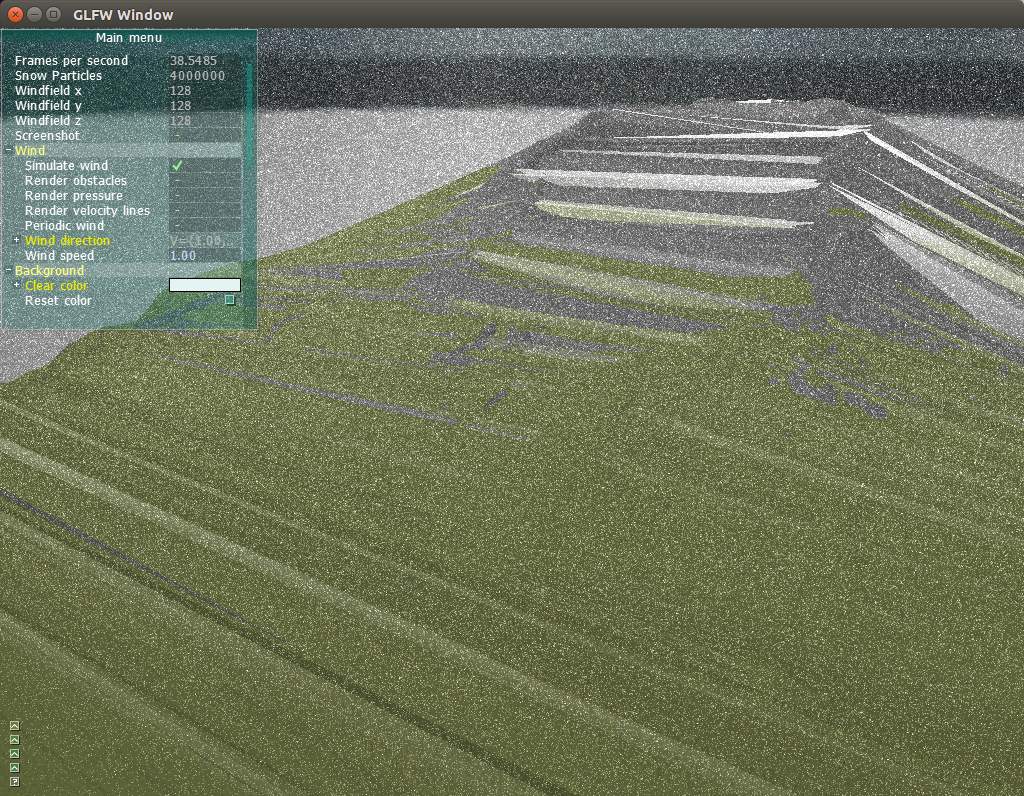
\includegraphics[width=\textwidth]{fig/smoothing}
\caption{Simulator with smoothing function enabled, showing erroneous results.}
\label{fig:smoothing}
\end{figure}

\pagebreak
%%=========================================
\subsection{Performance tests}
Table \ref{table:framerates} contains the framerates of the CUDA and OpenCL versions for various windfield sizes and particle counts. Profiling data is in the form of a bunch of screen shots, which can be seen in appendix \ref{appendix-b}.

\begin{table}[ht!]
  \begin{center}
    \begin{tabular}{| l | c | c | c |}
    \hline
    \diagbox{Windfield}{Snow particles} & 1 Million & 4 Million & 16 Million \\
    \hline
    32x32x32    & OpenCL: 298 & OpenCL: 113 & OpenCL: 34.0\\
                & CUDA: 336   & CUDA: 126   & CUDA: 45.5 \\
    \hline
    128x128x128 & OpenCL: 99 & OpenCL: 51.1 & OpenCL: 18.1\\
                & CUDA: 93   & CUDA: 52.8   & CUDA: 19.7 \\
    \hline
    256x256x256 & OpenCL: 22 & OpenCL: 17.7 & OpenCL: 10.7\\
                & CUDA: 18   & CUDA: 16.3   & CUDA: 10.4 \\
    \hline

    \end{tabular}
  \end{center}
  \caption{Framerates for various problem sizes}
  \label{table:framerates}
\end{table}

%%=========================================
\section{Discussion}
\subsection{Functional tests}
The only serious issue uncovered by functional testing was the erroneous results with ground smoothing enabled. The smoothing function works by comparing the height of a grid cell with the neighbors, and increasing or decreasing the height if the difference is, respectively, below or above a certain threshold. I can see two possible explanations for the observed behavior:
\begin{itemize}
\item The smoothing function is comparing the height not to that of the cell's neighbors, but to some more distant cell. This would indicate some sort of indexing error.
\item Race conditions. The change in height needs to happen after all threads have read the current height.
\end{itemize}

%%=========================================
\subsection{Performance tests}
% !TEX encoding = UTF-8 Unicode
%!TEX root = thesis.tex
% !TEX spellcheck = en-US
%%=========================================
\chapter{Discussion and Further Work}

\section{Discussion of Results}
\subsection{Functional Tests}
One serious issue uncovered by functional testing was the erroneous results with ground smoothing enabled. The smoothing function works by comparing the height of a grid cell with the neighbors, and increasing or decreasing the height if the difference is, respectively, below or above a certain threshold. I can see two possible explanations for the observed behavior:
\begin{itemize}
\item The smoothing function is comparing the height not to that of the cell's neighbors, but to some more distant cell. This would indicate some sort of indexing error.
\item Race conditions. The change in height needs to happen after all threads have read the current height.
\end{itemize}
The other issue was that snow particles seem to gradually disappear when the simulator is run for longer periods of time. If this was only visual, I would assume this was because they got stuck somewhere, unable to move. However, the fact that this effect is accompanied by a gradual increase in frame rate suggests that less and less computation is done. A possible explanation is that if lots of snow particles are stuck in one place, this increases data locality when reading the windfield, leading to the observed speedup.

%%=========================================
\subsection{Performance Tests}
From the frame rate data in table \ref{table:framerates} we see that the performance of the CUDA and OpenCL versions are comparable, but slightly different based on the parameters used. Larger wind fields lead to more similar results, while larger particle counts lead to better relative performance in the CUDA version. This would suggest that the OpenCL port lags the CUDA version in performance of the SnowSystem kernels. Anyone looking to improve the performance of the OpenCL version would do well to look here first.

The profiling data shows that for most settings the SnowSystem \texttt{part\_update} kernel takes as long or longer than the entire wind simulation (\texttt{wind\_advect}, \texttt{build\_solution}, \texttt{solve\_poisson} and \texttt{set\_boundary} five times each, and \texttt{wind\_project}). Rendering (the white space between the bars) takes a non-negligible amount of time as well.

%%=========================================
\section{Recommendations for Further Work}
\subsection{Bug Fixing}
Obviously, fixing the observed bugs should be a priority. A more sophisticated profiler (e.g. CodeXL) might be able to uncover the reason behind the disappearing snow particles by confirming or refuting my speculation about data locality. 

%%=========================================
\subsection{Optimization}
\subsubsection*{Asynchronous/Out-of-Order Execution}
OpenCL provides the possibility of letting the runtime decide the order of execution. All of the \texttt{clEnqueue...} family of functions have an output parameter \texttt{event}, as well as an input parameter \texttt{event\_list}. The event list is an array of event objects representing previous tasks that this task depends on. Thus one can create a \emph{task graph} representing all the dependencies between tasks, letting the runtime maximize efficiency by e.g. running kernel code and DMA transfers at the same time. This also has the benefit of sending a larger batch of commands to the GPU, reducing overhead.

The main, high-level dependencies in the Snow Simulator are:
\begin{itemize}
\item \texttt{part\_update} depends on the windfield calculation.
\item \texttt{update\_obstacles} depends on the changes to the heightmap from \texttt{part\_update} and \texttt{smooth\_ground}.
\end{itemize}
Since the windfield read by \texttt{part\_update} is in the form of a 3D texture, written at the very end of the windfield calculation, one could enqueue both the wind and snow simulation kernels at the same time, and only write the windfield texture after both were done. Something similar would have to be done to the heightmap updates.

\subsubsection*{3D Texture Writes}
There exists an optional OpenCL extension called \textbf{cl\_khr\_3d\_image\_writes}, which allows 3D textures to be written by kernel code. Currently the windfield is in the form of a vertex buffer object, which is copied to a 3D texture at the end of the windfield simulation. If the WindSystem kernels could write directly to this texture instead, one would eliminate this copy operation, as well as possibly improving data locality since textures are typically packed more densely than VBOs.

Support for this extension is limited, however. In particular, no current Nvidia hardware supports it. Consequently, one would have to check for this capability either at run time or compile time. Also, given the limited support, one might ask if it is worth the trouble at all.

\subsubsection*{Workgroup Sizes}
Currently, sizes and numbers of workgroups are fixed constants. The OpenCL Optimization Guide \citep{amd2014opencl} gives the minimum number of workgroups as being the number of compute units on the device. Beyond this, some tuning may be necessary to find the optimum. This tuning could potentially be done at automatically at runtime, writing the work partitioning settings to a file for future use.

\subsubsection*{Compiler Optimizations}
While OpenCL compilers typically optimize code quite aggressively, a number of potentially useful optimizations are turned off by default due to peculiarities in how floating point numbers work. As a simple example, the expressions 
\begin{equation*}
a \cdot b \cdot c \cdot a \cdot b \cdot c
\end{equation*}
and
\begin{equation*}
(a \cdot b \cdot c) ^ 2
\end{equation*}
which are equivalent when $a$, $b$ and $c$ are real numbers, are not equivalent when they are floating point numbers. Also, for full standards compliance one must check for numbers being NaN or Infinity, and pay attention to the signedness of zero.

It is possible to bypass all this, however, through the use of compiler flags. There are several, the most aggressive of which is \texttt{-cl-fast-relaxed-math}, which enables all ``unsafe'' math optimizations. To my knowledge, this will not impact the correctness of the Snow Simulator in any way, though one should of course check to be sure. 
% Include more chapters as required.
%%=========================================
\appendix
% !TEX encoding = UTF-8 Unicode
%!TEX root = thesis.tex
% !TEX spellcheck = en-US
%%=========================================

\chapter{Acronyms}
\begin{description}
\item[GPU] Graphics Processing Unit
\item[CPU] Central Processing Unit
\item[SIMD] Single Instruction, Multiple Data
\item[GPGPU] General-Purpose GPU
\item[API] Application Programming Interface
\item[APU] Accelerated Processing Unit
\item[VBO] Vertex Buffer Object
\end{description}
% !TEX encoding = UTF-8 Unicode
%!TEX root = thesis.tex
% !TEX spellcheck = en-US
%%=========================================

\chapter{Profiling Data}
\label{appendix-b}

\begin{figure}[ht!]
\centering
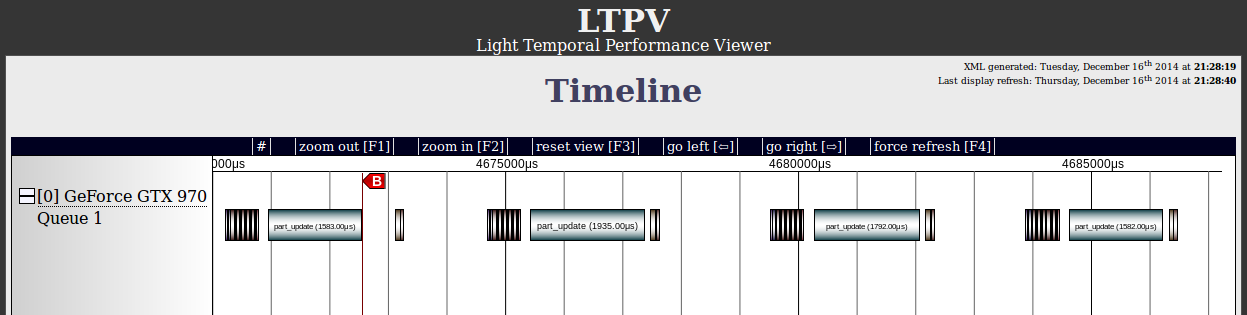
\includegraphics[width=\textwidth]{fig/profiling/1m_32}
\caption{Profiling data for 1 million particles, 32x32x32 windfield}
\label{fig:1m_32}
\end{figure}

\begin{figure}[ht!]
\centering
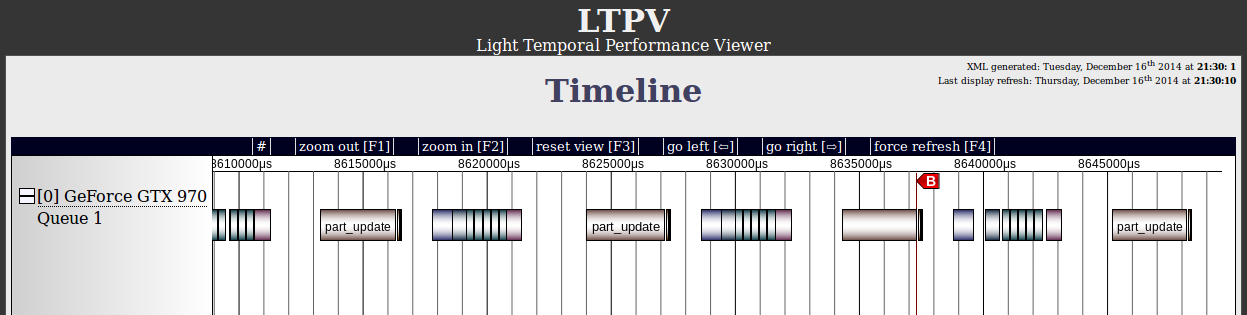
\includegraphics[width=\textwidth]{fig/profiling/1m_128}
\caption{Profiling data for 1 million particles, 128x128x128 windfield}
\label{fig:1m_128}
\end{figure}

\begin{figure}[ht!]
\centering
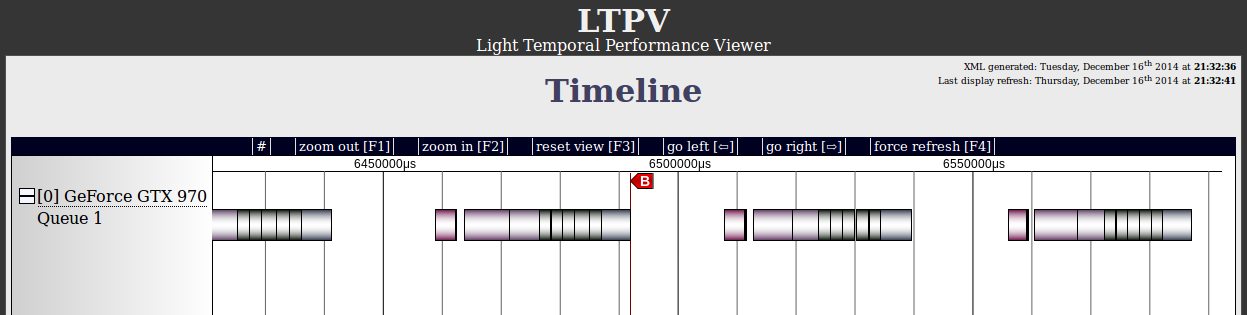
\includegraphics[width=\textwidth]{fig/profiling/1m_256}
\caption{Profiling data for 1 million particles, 256x256x256 windfield}
\label{fig:1m_256}
\end{figure}

\begin{figure}[ht!]
\centering
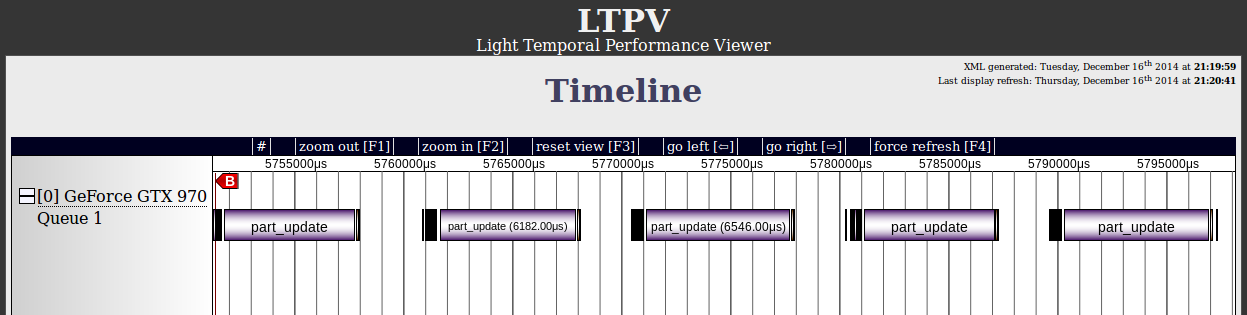
\includegraphics[width=\textwidth]{fig/profiling/4m_32}
\caption{Profiling data for 4 million particles, 32x32x32 windfield}
\label{fig:4m_32}
\end{figure}

\begin{figure}[ht!]
\centering
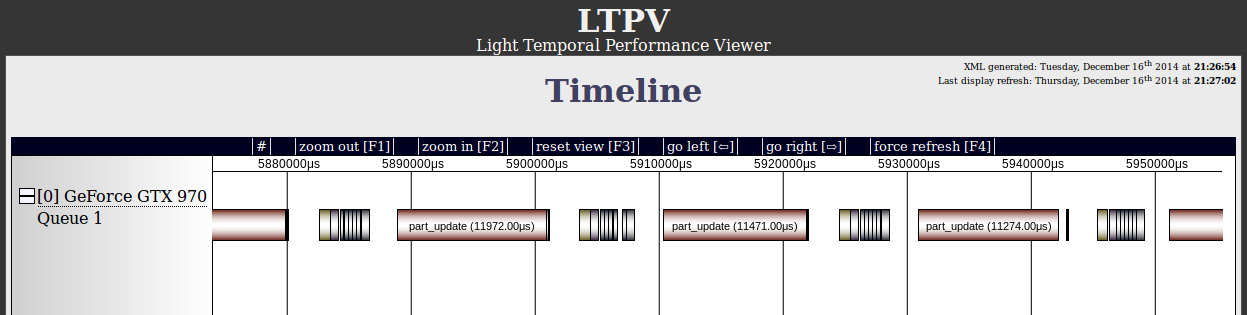
\includegraphics[width=\textwidth]{fig/profiling/4m_128}
\caption{Profiling data for 4 million particles, 128x128x128 windfield}
\label{fig:4m_128}
\end{figure}

\begin{figure}[ht!]
\centering
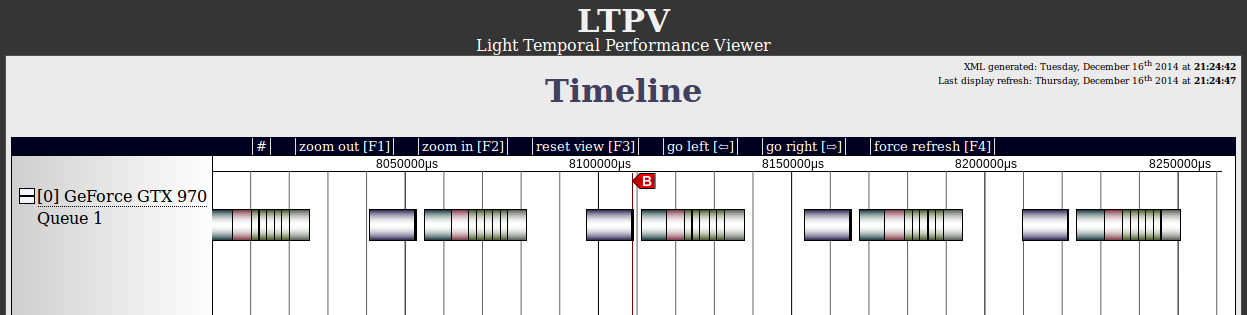
\includegraphics[width=\textwidth]{fig/profiling/4m_256}
\caption{Profiling data for 4 million particles, 256x256x256 windfield}
\label{fig:4m_256}
\end{figure}

\begin{figure}[ht!]
\centering
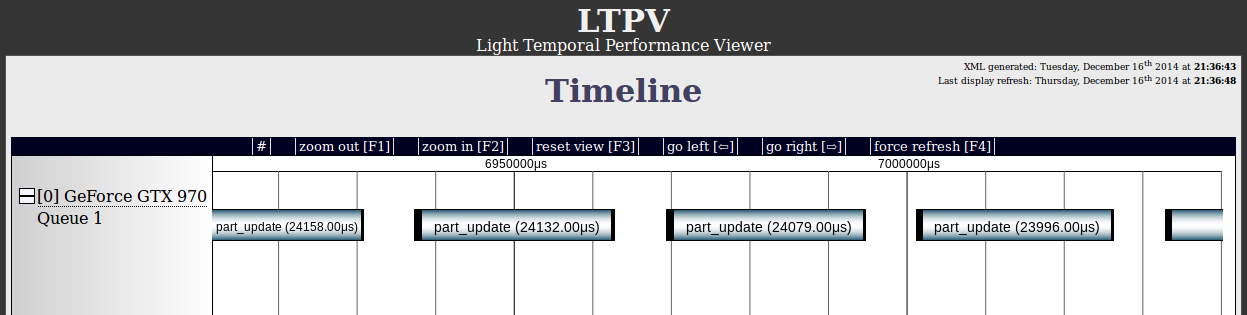
\includegraphics[width=\textwidth]{fig/profiling/16m_32}
\caption{Profiling data for 16 million particles, 32x32x32 windfield}
\label{fig:16m_32}
\end{figure}

\begin{figure}[ht!]
\centering
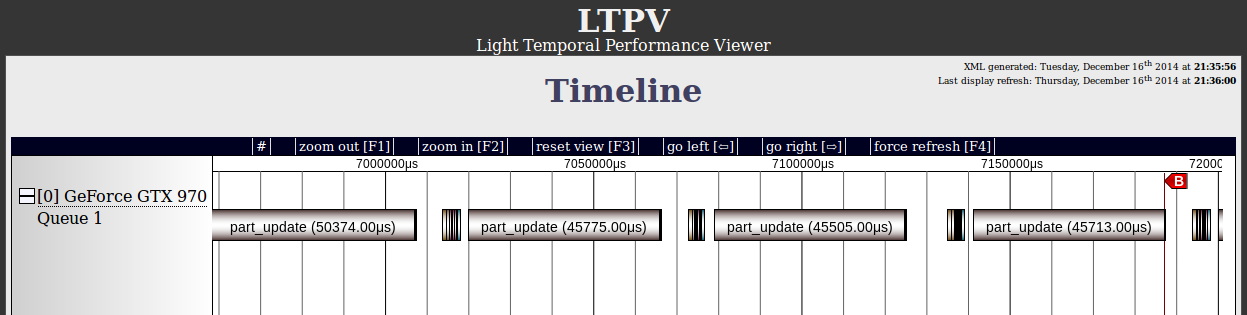
\includegraphics[width=\textwidth]{fig/profiling/16m_128}
\caption{Profiling data for 16 million particles, 128x128x128 windfield}
\label{fig:16m_128}
\end{figure}

\begin{figure}[ht!]
\centering
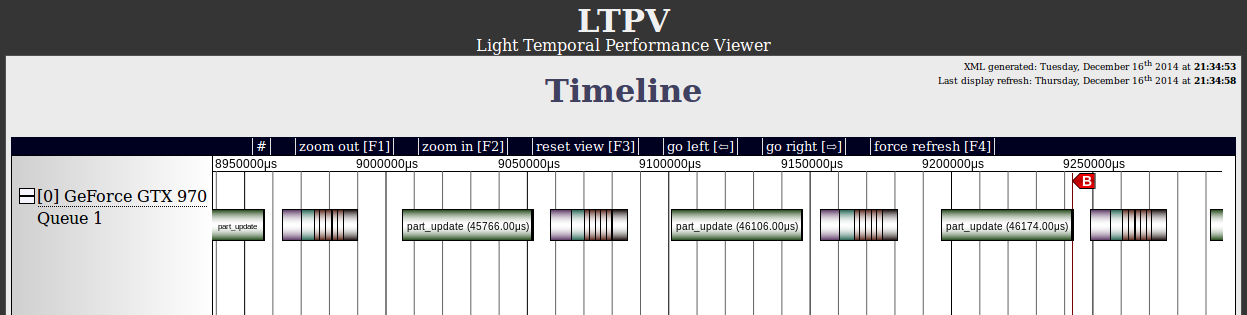
\includegraphics[width=\textwidth]{fig/profiling/16m_256}
\caption{Profiling data for 16 million particles, 256x256x256 windfield}
\label{fig:16m_256}
\end{figure}
% Include more appendices as required.
%%=========================================
\bibliographystyle{apa}
\addcontentsline{toc}{chapter}{\bibname}
\bibliography{refs}  
%%=========================================

\end{document}
